\documentclass{article}

\usepackage{amsmath}
\usepackage{amsthm}
\usepackage{amssymb}
\usepackage{color}
\usepackage{tikz}
\usetikzlibrary{shapes,arrows}
\usepackage{etoolbox}
\usepackage{url} % for urls in bibliography
\usepackage[parfill]{parskip} % no paragraph indents, leave blank line
\usepackage{graphicx}
\usepackage{subcaption}

% Need this to keep the space before theorems when using parfill parskip
% https://tex.stackexchange.com/questions/25346/wrong-spacing-before-theorem-environment-amsthm
\begingroup
    \makeatletter
    \@for\theoremstyle:=definition,remark,plain\do{%
        \expandafter\g@addto@macro\csname th@\theoremstyle\endcsname{%
            \addtolength\thm@preskip\parskip
            }%
        }
\endgroup

\title{Nitro Protocol}
\author{Tom Close}

\usepackage{mathtools}
\usepackage{bm}
\usepackage{stmaryrd} % for llbracket and rrbracket

\theoremstyle{definition}
\newtheorem{exmp}{Example}[section]
\newtheorem{defn}{Definition}[section]

\newcommand{\adj}[1]{\llbracket #1 \rrbracket} 
\newcommand{\enf}[1]{[#1]} 

\begin{document}

\maketitle

\section{Introduction}

A blockchain is a device that enables a group of adversarial parties to come to consensus over the contents of a shared ledger, without the presence of a trusted central authority. 
Whether using a proof-of-work or a proof-of-stake algorithm, this process has a cost both in terms of time and in terms of money.
For the Ethereum blockchain, this cost results in an effective limit of around 15 transactions per second being processed on the network.
When compared with the visa network, which can process on the order of 50,000 transactions per second, this limit supports the view that blockchains, in their current form, do not scale.

State channels offer a solution to the blockchain scaling problem.
A state channel can be thought of as a set of updatable agreements between a fixed set of participants determining how a given set of assets should be split between them.
The agreements are updated off-chain through the exchange of cryptographically signed messages between the participants according to some set of previously-agreed update rules. 
The assets in question are held in escrow on the blockchain, in such a way
that they can only be released according to the latest agreement from the state channel.
If the off-chain cooperative behaviour breaks down, for example if one party refuses to sign updates either by choice or due to unavailability, any of the parties can reclaim their share of the assets by presenting the latest agreement to the chain.
An exit game is required to give other parties the opportunity to present a later state, but all parties have the guarantee that they can reclaim their share of the funds within some finite time.

In addition to the increased throughput, state channels bring instant finality to transactions: the moment a channel update is received the participant knows that the assets transferred are now assigned to them.
They cannot access the assets immediately but they have the power to prevent any other party claiming those assets in the future.
The only requirement is that participants need to be live enough to engage in the exit game if an opponent attempts to exit an earlier state.
In practice, the requirement here is to check the chain periodically - at time intervals that are less than, but on the same order of magnitude as, the challenge duration in the exit game.

As the channel updates are created and exchanged off-chain, the channel-update throughput is limited only by the speed of constructing, signing and broadcasting the update.
Given that channel updates only needed to be communicated between participants and the system is therefore highly parallelizable, it is difficult to put a bound on the total transaction throughput of a system of state channels.
In practice the system is only limited by the on-chain operations required to move assets when opening and closing channels.

In this paper, we allow channels to be opened and closed off-chain. We enable the construction of efficient state channel networks.[TODO]

\section{Existing work}

Lightning and raiden
- payment channel networks
- directional

Celer
- directional but with multiple paths
- general conditions

Perun
- virtual payment channels (different from HTLCs)
- but using a validity time
- and then state channel networks
[Connext - have removed the time limit with a trade-off of trusting the hub - TODO: check this]

Counterfactual
- thinks about counterfactual instantiation
- also app instance on top, which we collaborated on
- possible to do meta-channels, but the details are not given in the paper and are still being finalized


Our contribution:
- like perun without the time limit


\section{Recap of ForceMove}

The ForceMove protocol describes the message format and the supporting on-chain behaviour
to enable generalized, $n$-party state channels on any blockchain that supports Turing-complete, general-purpose computation.
Here we give a brief overview of the protocol to the level required to understand
the rest of the paper. For a more comprehensive explanation please refer to \cite{}.

A ForceMove \textbf{state channel}, $\chi$, is defined by an ordered set of \textbf{participants}, $P = [p_0, ..., p_{n-1}]$ and a \textbf{channel nonce}, $k$, which is chosen by the participants.
The \textbf{channel address} is calculated by taking the last 20 bytes of the \texttt{keccak256}
hash of $(P, k)$.
We assume that channel addresses are unique, ignoring the possibility of finding an address
collision for channels with different sets of participants. 
We also assume that the space of channel addresses is disjoint from the space of all possible addresses generated from the public/private key algorithm, ignoring
the possibility of finding a collision here too.





Channel properties, the address of an on-chain \textbf{game library}, $L$,
challenge duration


\begin{table}[h]
  \begin{tabular}{|l|l|l|p{5cm}|}
    \hline
    \texttt{participants} & \texttt{address[]} & $P$ & The addresses used to sign updates to the channel. \\ \hline
    \texttt{nonce} & \texttt{unit256} & $k$ & Chosen to make the channel's address unique. \\ \hline
    \texttt{gameLibrary} & \texttt{address} & $L$ & The address of the gameLibrary, which defines the transition rules for this channel \\ \hline
    \texttt{challengeDuration} & \texttt{unit256} & $\eta$ & \\ \hline
    \texttt{turnNum} & \texttt{unit256} & $i$ & Increments as new states are produced. \\ \hline
    \texttt{balances} & \texttt{(address, uint256)[]} & $\beta$ & Current \textit{outcome} of the channel. \\ \hline
    \texttt{isFinal} & \texttt{bool} & $f$ & \\ \hline
    \texttt{data} & \texttt{bytes} & $\delta$ & \\ \hline
    \texttt{v} & \texttt{uint8} & &  ECDSA signature of the above arguments by the moving participant. \\ \cline{1-2}
    \texttt{r} & \texttt{bytes32} & & \\ \cline{1-2}
    \texttt{s} & \texttt{bytes32} & & \\ \hline
  \end{tabular}
  \caption{ForceMove state format}
  \label{table:force-move-state}
\end{table}

A ForceMove \textbf{state}, $\sigma_\chi^i(\beta, f, \delta)$, is specified by \textbf{turn number}, $i$,
a set of \textbf{balances}, $\beta$, a boolean flag \textbf{finalized}, $f \in \{T, F\}$, and
a chunk of unstructured \textbf{game data}, $\delta$, that will be interpreted by the game library. The
balances can be thought of as an ordered set of $(\texttt{address}, \texttt{uint256})$ pairs,
which specify how any funds allocated to the channel should be distributed if the channel 
were to finalize in the current state.

In order for a state, $\sigma_\chi^i$, to be valid it must be signed by participant, $p_j$,
where $j = i \% n$ is the remainder mod $n$. This requirement specifies that participants
in the channel must take turns when signing states.

The game library is responsible for defining a set of states and allowed transitions that
in turn define the `application' that will run inside the state channel. It does this by
defining a single boolean function, $t_L(i, \beta, \delta, \beta', \delta') \rightarrow \{ T, F\}$.
This function is used to derive an overall boolean transition function, $t$, specifying whether
a transition between two states is permitted under the rules of the protocol:
\begin{align*}
  t(\sigma_\chi^i(\beta, f, \delta), \sigma_{\chi'}^j(\beta', f', \delta') ) \Leftrightarrow &
    \chi = \chi'
    \wedge j = i + 1
    \wedge \\
    & [ (\neg f \wedge \neg f' \wedge j \leq 2n \wedge \beta = \beta' \wedge \delta = \delta') \vee \\
    & (\neg f \wedge \neg f' \wedge j > 2n \wedge t_L(n, \beta, \delta, \beta', \delta')) \vee \\
    & (f' \wedge \beta = \beta' \wedge \delta' = 0) ]
\end{align*}

In all transitions the channel properties must remain unchanged and the turn number must increment.
There are then three different modes of operation. The first mode applies in the first $2n$
states (assuming none of these are finalized) and in this mode the balances and game data
must remain unchanged. As we will see later, these states exist so that the channel can be
funded safely. We refer to the first $n$ states as the \textbf{pre-fund setup} states and
the subsequent $n$ as the \textbf{post-fund setup} states. The second mode applies to the
`normal' operation of the channel, when the game library is used to determine the allowed
transitions. The final mode concerns the finalization of the channel: at any point the current
participant can choose to exit the channel and lock in the balances in the current state.
Once this happens the only allowed transitions are to additional finalized states. Because
of this, we have no further use for the game data, $\delta$, so can remove this from the state.
Once a sequence of $n$ finalized states have been produced the channel is considered closed. We
call this sequence of $n$ finalized states a \textbf{conclusion proof}, which we will write $\bm{\sigma}^*$.

\begin{figure}[ht]
  \centering
    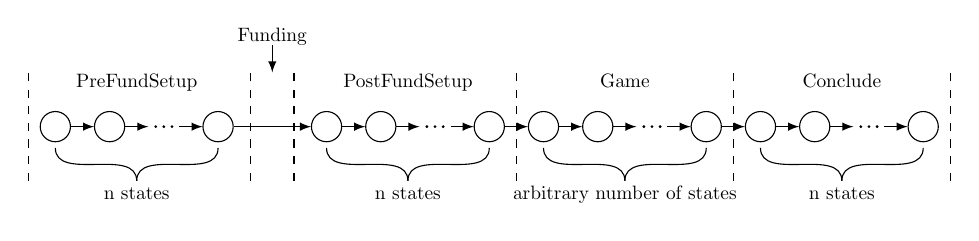
\begin{tikzpicture}[x=28pt,y=28pt,scale=0.7, every node/.style={transform shape}]
        \newcommand{\paperdiagram}[3]{%
            \begin{scope}[shift={(#1,0)}]
                % Circle
                \foreach \n in {0,1,3} {\node[circle,draw,text width=10pt,inner sep=0pt] (N\n#1) at (\n,0) {\strut};}
                % Transparent circle
                \foreach \n in {2} {\node[circle,draw,text width=10pt,inner sep=0pt,white] (N\n#1) at (\n,0) {\strut};}
                % Dots
                \foreach \n in {1.85,2,2.15} {\fill (\n,0) circle (0.8pt);}
                % Arrows
                \foreach \x [remember=\x as \lastx (initially 0)] in {1,2,3}{\draw[-latex] (N\lastx#1) -- (N\x#1);}
                % Under brackets with label #3
                \foreach \n in {0,3} {\draw ([shift={(0,-3pt)}]N\n#1.south) to[out=270,in=90] (1.5,-1) node[inner sep=1pt] (P) {\strut};}
                \node at (P.south) {\strut#3};
                % Upper label #2
                \node at (1.5,0.8) {\strut#2};
            \end{scope}
        }
        % Diagram nodes
        \paperdiagram{0}{PreFundSetup}{n states}
        \paperdiagram{5}{PostFundSetup}{n states}
        \paperdiagram{9}{Game}{arbitrary number of states}
        \paperdiagram{13}{Conclude}{n states}
        % Arrows between single diagram node
        \foreach \x [remember=\x as \lastx (initially 0)] in {5,9,13}{\draw[-latex] (N3\lastx) -- (N0\x);}
        % Vertical dashed
        \foreach \n in {-0.5,3.6,4.4,8.5,12.5,16.5} {\draw[dashed] (\n,-1) --++(90:2);}
        % Funding arrow
        \draw[latex-] (4,1) --++(90:0.5) node[at end,above,inner sep=0pt] {Funding};
    \end{tikzpicture}

    \caption{
        Overview of the stages of collaborative play in the ``happy path'' case. Note that
        the allowed transitions from $\texttt{PRE/POSTFUNDSETUP} \mapsto \texttt{CONCLUDE}$ are
        omitted from the diagram.
    }
    \label{fig:game-overview}
\end{figure}


\subsection{On-chain operations}

todo: intro
We will talk about the adjudicator as though it is a single contract but don't intend to take a position on how it should be constructed by doing so; it is likely that in practice the adjudicator functionality will be provided by a set of interacting contracts.

We will refer to the on-chain contract as the \textbf{adjudicator}, which we will write $\adj{S}$, where $S$ represents the contract's internal state. The state consists of three collections: the allocations, the outcomes and the challenges, each of which is keyed by a channel address. 

The \textbf{allocations} collection is an \texttt{(address -> uint256)} mapping that records the total funds allocated to a given channel. We write $\adj{\alpha_\chi(x)}$ to represent an adjudicator where $x$ is allocated to channel $\chi$.

The \textbf{outcomes} collection assigns channels to one of two different modes: channels are either undecided or decided. We use the symbol $\cdot$ to represent undecided channels, so that $\adj{\beta_\chi(\cdot)}$ represents an adjudicator where the outcome of channel $\chi$ is undecided. For channels with outcomes that are decided, the outcomes collection maps the channel address to an ordered set of \texttt{(address, uint256)} pairs - exactly the same format as the channel balances. We write $\adj{\beta_\chi(X: x, Y: y)}$ for an adjudicator where the outcome for channel $\chi$ is decided and sends $x$ to address $X$ and $y$ to address $Y$.

The \textbf{challenges} collection records whether there is an active challenge on a given channel. We write $\adj{\kappa_\chi(\tau, \sigma)}$ for the case where there's an active challenge on channel $\chi$ challenging with state $\sigma$ and expiring at time $\tau$. We write $\adj{\kappa_\chi(\cdot)}$ in the case where there is no open challenge and $\adj{\kappa_\chi(\times)}$ in the case where a challenge has expired (and thus no further challenges are possible). An efficient real-world implementation would most likely store the challenges as part of the outcomes collection, but we have chosen to treat them as separate concepts for the purpose of this paper.

Note that while using the above notation in the rest of the paper, we will suppress the unimportant parts of the state, with the understanding that these parts of the state remain unchanged. It is also understood that zero entries can be ignored in outcomes, so that $\beta(a_1: 0, a_2:x_2,...) \equiv \beta(a_2:x_2, ...)$.

We now move on to describing the operations supported by the adjudicator. The first operation we look at is the \textbf{deposit}:
\begin{align*}
D_\chi(x) \adj{\alpha_\chi(y)} \rightarrow \adj{\alpha_\chi(x + y)}
\end{align*}
The deposit can be called by anyone and results in an increase in the allocation for the given channel.

There is also a \textbf{withdrawal} operation that can be used by anyone with the private key for address $A$ to withraw funds allocated to $A$ by an outcome:
\begin{multline*}
W_A(x) \adj{\alpha_\chi(x_\alpha)\beta_\chi(A: x_\beta, ...)} \rightarrow \\
\begin{cases}
  \adj{\alpha_\chi(x_\alpha - x)\beta_\chi(A: x_\beta - x, ...)} &
  \text{if } x \leq x_\alpha, x_\beta  \\
  \adj{\alpha_\chi(x_\alpha)\beta_\chi(A: x_\beta, ...)} &
  \text{otherwise}
\end{cases}
\end{multline*}
In order to call the withdraw, the caller needs to sign the withdraw operation using the private key of the address the withdrawal is from. Thus it is not possible to call the withdraw operation for an address that corresponds to a state channel, as these addresses were generated from a hash of the channel's properties and not from a public/private key pair.

The next operation is the \textbf{force-move} which is used to register a challenge for a channel $\chi$ if no challenge (active or expired) currently exists:
\begin{align*}
FM(\tau, \bm{\sigma}_i^{i+n-1}) \adj{\kappa_\chi(x)} \rightarrow 
\begin{cases}
  \adj{\kappa_\chi(\tau + \eta, \sigma^{i+n-1})} &
  \text{if } x = \cdot \wedge t(\bm{\sigma}_i^{i+n-1}) \\
  \adj{\kappa_\chi(x)} &
  \text{otherwise}
\end{cases}
\end{align*}
where we write $\bm{\sigma}_i^{i+n-1}$ to represent the sequence of states $\sigma^i \dots \sigma^{i+n-1}$ and $t(\bm{\sigma}_i^{i+n-1}) = t(\sigma^{i}, \sigma^{i+1}) \wedge \dots \wedge t(\sigma^{i+n-2}, \sigma^{i+n-1})$.

The intent of a force-move is to get the next participant to provide their next move to the adjudicator. To do this they can call the \textbf{respond} method, providing their next state:
\begin{align*}
R(\tau', \sigma^{i+1})\adj{\kappa(\tau, \sigma^i)} \rightarrow
\begin{cases}
  \adj{\kappa_\chi(\cdot)} & \text{if } \tau' < \tau \wedge t(\sigma^i, \sigma^{i+1}) \\
  \adj{\kappa(\tau, \sigma^i)} &
  \text{otherwise}
\end{cases}
\end{align*}
Once the challenge is cancelled it is removed from the adjudicator and the channel operation can continue off-chain. The force-move paper \cite{} outlines a couple of alternative ways (\textbf{refute} and \textbf{respond-with-alternative-move}) to respond to a force-move. While these are important for the ForceMove protocol, we will not need them in this paper, so will not go over them here.

If the opponent does not respond to the challenge before the challenge expiry time, $\tau$, then a \textbf{timeout} occurs:
\begin{align*}
\Theta(\tau + \epsilon) \adj{\kappa(\tau, \sigma_\chi(\beta_\chi, \delta))} \rightarrow \adj{\beta_\chi \kappa_\chi(\times)}
\end{align*}
Unlike the other operations on this list, the timeout operation is not triggered by a
blockchain transaction. Instead the operation happens automatically when the block time
exceeds the expiry time stored in the challenge. In practice, there will not be any change 
to the state stored in the contract when the operation occurs - just a change to the
interpretation of that state. 

The final operation is the \textbf{conclude} operation, which enables the immediate creation of a channel outcome from a conclusion proof, $\bm{\sigma}^*(\beta)$ including in the case where there is an active challenge:
\begin{align*}
C(\tau, \bm{\sigma}^*(\beta)) \adj{\kappa_\chi(x)} \rightarrow 
\begin{cases}
  \adj{\kappa_\chi(\times)} & \text{if } x = \times \\
  \adj{\beta_\chi(\beta) \kappa_\chi(\times)} &
  \text{otherwise}
\end{cases}
\end{align*}
The conclude operation enables instant withdrawals in the case the channel is concluded collaboratively off-chain.

\section{Reasoning about State Channels}

Develop the reasoning and logic for the rest of the paper.
We introduce these concepts using the ForceMove framework but they are the central concepts of all state channel logic and can be applied to all state channel systems.

State channels enable value to be transferred off-chain.
How does this work when the chain is the record of value?
Consider value to be transferred off-chain, when the right to obtain
that value on-chain is transferred.
To understand a state channel it's therefore key to understand the capabilities our current set of states and private information affords us.

This involves not only reasoning about the states and private information they hold and their knowledge about what other players hold. In doing this
we don't track 
- assume that any state you have received is public
- assume that any state that is sent is public

In ForceMove, the only way a channel can affect the on-chain funds is via
the channel balances, $\beta$, being placed in the adjudicator. We will
refer to these final balances as the \textbf{outcome} of the channel and
will refer to their placement in the adjudicator as \textbf{finalizing} the outcome. As we saw in the previous section, there are two ways to register an outcome with the adjudicator: (i) by calling the force-move operation which no-one responds to before the expiry time or (ii) by calling the conclude operation with a conclusion proof.

We will simplify the analysis with the following assumptions:
\begin{itemize}
\item \textbf{Availability}: Given $\epsilon > 0$ and time $t$ it is always possible for any party to perform an on-chain operation in the interval $(t, t+\epsilon)$.
\item \textbf{Responsiveness}(?): All on-chain operations are immediately visible to all parties.
\item \textbf{Zero Gas}: On-chain operations are free.
\end{itemize}
In practice, we approximate the availability and responsiveness assumptions by ensuring that $\epsilon$ is sufficiently large, so that the assumption holds in practice. We do this by choosing the the channel timeout and requirements around how frequently participants should need to check the chain. The Zero Gas assumption means that we don't take the cost of operations into account when analysing the value of states. This is a good approximation when the gas costs are small compared with the value of the states - other cases require a more detailed analysis. This should be the subject of future research but falls outside the scope of this paper.

\subsection{Finalizable Outcomes}

finalizability of an outcome, $\beta$ is \textbf{finalizable} by $p$:
* it is possible for $p$ to finalize $\beta$ in the adjudicator $\adj{\beta_\chi(\beta)}$ and no-one else can stop them. We write this $\enf{\beta}_p$.

Example: $p$ is the next player to move

It is possible for an outcome to be finalizable for multiple players at the same time:

Example: a single conclusion proof exists

Example: after the post fund setup

Note that it is also possible for more than one outcome to be finalizable by a player. We will see an example of this later. It follows from the definition of finalizability that it is impossible to simultaneously have one player with more than one finalizable outcome and more than one player at least one finalizable outcomes. 

It's also possible to get into a state where no outcomes are finalizable by anyone. This is usual undesirable and a sign that something somewhere has gone wrong. An example of this is the case where two different conclusion proofs exist.


\subsection{Enabled Outcomes}

It is often the case that a given player, $p$, will have no finalizable outcomes at a given point in time. In this case we instead look at the set of \textbf{enabled} outcomes for $p$, which we write $\{\beta_1, ... \beta_i\}_p$. The enabled outcomes are the set of all outcomes of the channel that are possible up until $p$ signs their next state. They are the outcomes that were enabled by $p$'s last signature.

All the possible ways the channel can end before they take their next turn - that they can't control(?).

The set of enabled outcomes has the property that $p$ can cause one of them to be registered with the adjudicator (e.g. through repeated force-moving) but cannot choose which one.

Sometimes a player might have incomplete knowledge, so they are not able to calculate the possible states. In this case the enabled outcomes should include all possible states as far as the player can tell. An example of this occurs in commit-reveal schemes: say two players are playing a guessing game where player A commits to a value, player B makes a guess and then player A reveals whether they were right. At the point where B has just made their guess, the outcome is determined but B does not yet know what it is. In this case, the enabled outcomes for B should include the outcome where B was correct and the outcome where B was incorrect.

If a player has finalizable outcomes, they do not have any enabled outcomes.
If a player has only one enabled outcome then, by the definitions, it is an finalizable outcome: $\{\beta \}_p \equiv \enf{\beta}_p$. 


\subsection{The Consensus Game}

The Consensus Game is an important ForceMove application, which we will use heavily in the rest of the paper due to its special properties regarding outcome finalizability. In this section we introduce transition rules and explore these properties.

Like all ForceMove applications, the transition rules for the Consensus Game are specified by a game library, $L_C$, which defines the transition function, $t_{L_C}$, in terms of the turn number, $i$, the balances, $\beta$ and the game data $\delta$. $\delta = (j, x)$, where $j$ is the \textit{consensus counter} and $x$ is the \textit{proposed balances}. 
\begin{align*}
  t_{L_C}(i, \beta, (j, x), \beta', (j', x')) \Leftrightarrow
    [ & (j=n-1 \wedge j'= 0 \wedge \beta' = x = x')  \vee \\
    & (j < n-1 \wedge j' = j+1, \beta = \beta', x = x') \vee \\
    & (j'=0, \beta = \beta') ]
\end{align*}
For a given $\beta$, the consensus counter will increase from $0\dots (n-1)$ as the participants sign off on the new balances. Once all participants have signed, consensus has been reached and the channel's balances are updated.

  \begin{align*}
    \sigma^{i}(\beta, (0, \beta)) & \approx [\beta]_P \\
    \sigma^{i+1}(\beta, (0, \beta')) & \approx \{\beta'\}_{p_0}[\beta]_{p_1, ..., p_{n-1}} \\
    \sigma^{i+2}(\beta, (1, \beta')) & \approx \{\beta'\}_{p_0, p_1}[\beta]_{p_2, ..., p_{n-1}} \\
    &\vdots\\
    \sigma^{i+n-1}(\beta, (n-1, \beta')) & \approx [\beta', \beta]_{p_{n-1}} \\
    \sigma^{i+n}(\beta', (0, \beta')) & \approx [\beta']_{P} \\
  \end{align*}

Safe update theorem

This allows us to change one channel at a time


\section{Turbo Protocol}

Turbo protocol is a small extension to ForceMove that allows multiple ForceMove state
channels between a the same set of participants to be supported by a single on-chain
state deposit.

* parallelized
* open and close off-chain
* generalisation of addresses

In Turbo the ForceMove withdrawal operation, $W_A(x)$, is replaced with two operations: a
\textbf{transfer} operation, $T_{A,B}(x)$, and a modified withdrawal operation, $W'_B(x)$.
The original ForceMove withdrawal can be recovered as $W_A(x) = W'_B(x)T_{A,B}(x)$.

The modified withdrawal operation, $W'_A(x)$, allows withdrawal directly from the funds
held for address, $A$. The operation requires knowledge of the private key of $A$ and is
therefore not possible for addresses that correspond to state channels. The operation has
the following effect on the on-chain state:
\begin{align*}
W'_A(x) \adj{\alpha_A(x')} \rightarrow \adj{\alpha_A(x'-x)}
\end{align*}

The transfer operation, $T_{A,B}(x)$, is an instruction to transfer funds currently allocated
to address $A$ to address $B$, according to the outcome of channel $A$:
\begin{multline*}
T_{AB}(x) \adj{\alpha_A(x_\alpha)\beta_A(B:x_\beta, \dots)} \rightarrow \\
  \begin{cases}
      \adj{\alpha_A(x_\alpha - x)\alpha_B(x)\beta_A(B:x_\beta - x, \dots)} & 
      \text{if } x \leq x_\alpha, x_\beta \\
      \adj{\alpha_A(x_\alpha)\beta_A(B:x_\beta, \dots)} &
      \text{otherwise}
  \end{cases}
\end{multline*}

\subsection{Ledger channels}

Rules of the consensus game

\subsection{Opening a sub-channel}

Want to open the channel, $\chi$, where $A$ and $B$ have initial balances $a' \leq a$ and $b' \leq b$ respectively. Both players start by signing a pre-fund setup for $\chi$ leaving us in the state:

Note that we also have $S_3 \sim \omega_A(a)\omega_B(b)$. In order to transition to this state with the collaboration game, we have to transition through 

We start with a ledger channel 
\begin{align*}
S_1 &= \adj{\alpha_L(a+b)} &&\enf{\beta_L(A: a, B: b)}_{A, B} & \\
S_2 &= \adj{\alpha_L(a+b)} &&\enf{\beta_L(A: a, B: b)}_{A, B}&\enf{\beta_\chi(A: a', B: b')}_{A, B} \\
S_3 &= \adj{\alpha_L(a+b)} &&\enf{\beta_L(A: a-a', B: b-b', \chi: a' + b')}_{A, B}&\enf{\beta_\chi(A: a', B: b')}_{A, B}
\end{align*}

\subsection{Closing a sub-channel off-chain}

\begin{align*}
S_1 &= \adj{\alpha_L(x)} &&\enf{\beta_L(A: a, B: b, \chi: a' + b')}_{A, B}&\enf{\beta_\chi(A: a', B: b')}_{A, B}\\
S_2 &= \adj{\alpha_L(x)} &&\enf{\beta_L(A: a + a', B: b + b')}_{A, B}&\enf{\beta_\chi(A: a', B: b')}_{A, B} \\
S_3 &= \adj{\alpha_L(x)} &&\enf{\beta_L(A: a + a', B: b + b')}_{A, B} & 
\end{align*}
where $x = a + a' + b + b'$.

\subsection{Topping up a ledger channel}

\begin{align*}
S_1 &= \adj{\alpha_L(a + b)} &&\enf{\beta(A: a, B: b)}_{A, B} \\
S_2 &= \adj{\alpha_L(a + b)} &&\enf{\beta(B: b, A: a + a')}_{A, B} \\
S_3 &= D_L(a')\adj{\alpha_L(a + b)} &&\enf{\beta(B: b, A: a + a')}_{A, B} \\
S_4 &= \adj{\alpha_L(a + b + a')} &&\enf{\beta(B: b, A: a + a')}_{A, B}
\end{align*}

\subsection{Partial checkout from a ledger channel}

\begin{align*}
S_1 &= \adj{\alpha_L(x)} &&\enf{\beta_L(B: b, A: a, \chi: c)}_{A, B} & \\
S_2 &= \adj{\alpha_L(x)} &&\enf{\beta_L(B: b, A: a, \chi: c)}_{A, B} & \enf{\beta_{L'}(B: b, A: a - a', \chi: c)}_{A, B}\\
S_3 &= \adj{\alpha_L(x)} &&\enf{\beta_L(L': x-a', A: a)}_{A, B} & \enf{\beta_{L'}(B: b, A: a - a', \chi: c)}_{A, B}\\
S_4 &= \adj{\alpha_L(x)\beta_L(L': x-a, A: a)} && & \enf{\beta_{L'}(B: b, A: a - a', \chi: c)}_{A, B}\\
S_5 &= \adj{\alpha_L'(x-a)\alpha_A(a)} && & \enf{\beta_{L'}(B: b, A: a - a', \chi: c)}_{A, B}\\
\end{align*}


\section{Nitro Protocol}

Nitro protocol is an extension to Turbo protocol that enables a group of parties to open a state channel without having a mutual on-chain deposit,
provided they do all have an on-chain deposit with a shared third party.

In order to enable virtual channels, we need to add a new type of channel - the \textbf{guarantor channel} - to the framework. We will distinguish these from regular channels by referring to regular channels as \textbf{balance channels} from now on.

Guarantor channels differ from balance channels in that both the channel and the outcome stores one extra property - \textbf{gurantorFor} - which stores the address of the channel that they guarantee. Their outcomes are also interpreted differently. The outcome of a guarantor channel, $A$, which guarantees channel $B$ is written $\gamma_{A, B}(C_1: x_1, C_2: x_2, \dots)$. This outcome means that $A$ will cover $B$'s debt to $C_1$ up-to an amount $x_1$, then $B$'s debt to $C_2$ up-to an amount $x_2$ and so on.

We introduce another on-chain operation $G_{A, C}(x)$ which involves claiming an amount $x$ from $A$'s guarantee for $C$. The operation is defined as follows:
\begin{multline*}
G_{AC}(x) \adj{\alpha_A(x_\alpha)\gamma_{A,B}(C:x_\gamma, \dots)\beta_B(\dots, C:x_\beta, \dots)} \rightarrow \\
  \begin{cases}
      \adj{\alpha_A(x_\alpha - x)\alpha_C(x)\gamma_{A,B}(C:x_\beta -x, \dots)\beta_B(\dots, C:x_\beta - x, \dots)} \\
      \hspace{7cm} \text{if } x \leq x_\alpha, x_\beta, x_\gamma \\
      \adj{\alpha_A(x_\alpha)\gamma_{A,B}(C:x_\gamma, \dots)\beta_B(\dots, C:x_\beta, \dots)} \\
      \hspace{7cm} \text{otherwise}
  \end{cases}
\end{multline*}
TODO: rewrite this and explain.

\begin{table}[h]
  \begin{tabular}{|l|l|l|p{5cm}|}
    \hline
    \texttt{participants} & \texttt{address[]} & $P$ & The addresses used to sign updates to the channel. \\ \hline
    \texttt{gameLibrary} & \texttt{address} & $L$ & The address of the gameLibrary, which defines the transition rules for this channel \\ \hline
    \texttt{nonce} & \texttt{unit256} & $k$ & Chosen to make the channel's address unique. \\ \hline
    \texttt{challengeDuration} & \texttt{unit256} & $\eta$ & \\ \hline
    \texttt{turnNum} & \texttt{unit256} & $i$ & Increments as new states are produced. \\ \hline
    \texttt{guarantorFor} & \texttt{address} &  & Target channel for guarantee channels. Equal to 0 for balance channels. \\ \hline
    \texttt{balances} & \texttt{(address, uint256)[]} & $\beta$ or $\gamma$ & Current \textit{outcome} of the channel. \\ \hline
    \texttt{isFinal} & \texttt{bool} & $f$ & \\ \hline
    \texttt{data} & \texttt{bytes} & $\delta$ & \\ \hline
    \texttt{v} & \texttt{uint8} & &  ECDSA signature of the above arguments by the moving participant. \\ \cline{1-2}
    \texttt{r} & \texttt{bytes32} & & \\ \cline{1-2}
    \texttt{s} & \texttt{bytes32} & & \\ \hline
  \end{tabular}
  \caption{ForceMove state format}
  \label{table:force-move-state}
\end{table}

\subsection{Virtual Channels}

Virtual channels is this: 
Why? Equivalent for A, B and C

\begin{figure}[h]\centering
  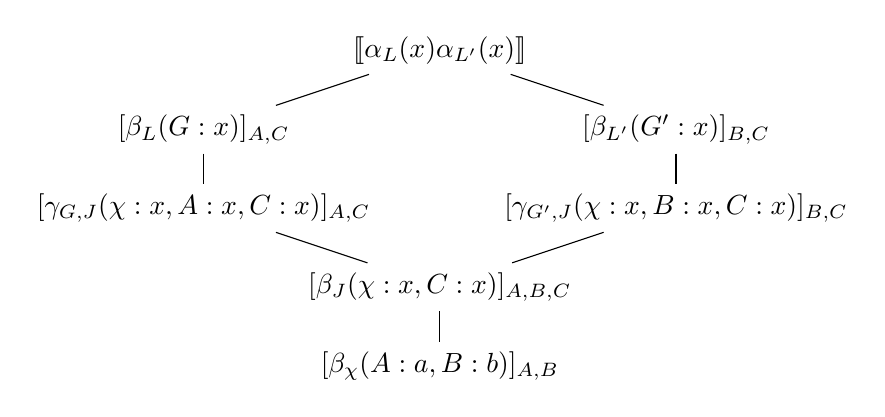
\begin{tikzpicture}[x=3cm,y=1cm]

    % Specification of nodes (position, etc.)
    \node (a0) at (0,0) { $\adj{\alpha_L(x)\alpha_{L'}(x)}$ };
    \node (b0) at (-1,-1) { $\enf{\beta_L(G: x)}_{A, C}$ };
    \node (b1) at (1,-1) { $\enf{\beta_{L'}(G': x)}_{B, C}$ };
    \node (g0) at (-1,-2) { $\enf{\gamma_{G, J}(\chi: x, A: x, C: x)}_{A, C}$ };
    \node (g1) at (1,-2) { $\enf{\gamma_{G', J}(\chi: x, B: x, C: x)}_{B, C}$ };
    \node (j) at (0,-3) { $\enf{\beta_J(\chi: x, C: x)}_{A,B,C}$ };
    \node (c) at (0,-4) { $\enf{\beta_\chi(A: a, B: b)}_{A,B}$ };

    \begin{scope}[-]
      \tikzstyle{every node}=[draw=none,below]
      \draw (a0) to (b0);
      \draw (a0) to (b1);
      \draw (b0) to (g0);
      \draw (b1) to (g1);
      \draw (g0) to (j);
      \draw (g1) to (j);
      \draw (j) to (c);
    \end{scope}

  \end{tikzpicture}
\caption{Ledger channels, $x = a + b$}\label{fig:modes}
\end{figure}

There is a configuration where we can support virtual channels.
They can be opened and closed off-chain.

Want to fund a channel $\chi$ between A and B, for which we have state $\enf{\beta_\chi(A: x, B:y)}_{A,B}$. We have channels $L$ and $L'$ with participants $\{A, C\}$ and $\{B, C\}$ respectively. We assume these channels start in states $\enf{\beta_L(A:x, C:)}$

\begin{align*}
  \adj{\alpha_L(x)\alpha_{L'}(x)} \quad \enf{\beta_L(A: a, C: b)}_{A,C} \quad \enf{\beta_{L'}(B:b, C:a)}_{B, C}
\end{align*}

The offload
\begin{align*}
  & \adj{\alpha_L(x)\beta_L(G: x)\gamma_{G,J}(\chi: x, C: x)\beta_J(\chi: x, C: x)\beta_\chi(A: a, B: b)}\\ 
  & \begin{aligned}
   \xrightarrow{T_{L,G}(x)} & \adj{\alpha_G(x)\gamma_{G, J}(\chi: x, C: x)\beta_J(\chi: x, C: x)\beta_\chi(A: a, B: b)} \\
   \xrightarrow{G_{G, J, \chi}(a)} & \adj{\alpha_\chi(x)\beta_\chi(A: a, B: b)\gamma_{G, J}(C: x)\beta_J(C: x)} \\
   \xrightarrow{T_{\chi, A}(a)} & \adj{\alpha_A(a)\alpha_\chi(b)\beta_\chi(B: b)\gamma_{G, J}(C: x)\beta_J(C: x)} \\
   \approx & \alpha_A(a)
  \end{aligned}
\end{align*}

\subsection{Opening a virtual channel}
We let
\begin{align*}
l_0 &= \enf{\beta_L(A:a, C: b)}_{A, C} &
l_1 &= \enf{\beta_L(G: x)}_{A, C} \\
l'_0 &= \enf{\beta_{L'}(B:b, C: a)}_{B, C} &
l'_1 &= \enf{\beta_{L'}(G': x)}_{B, C} \\
j_0 &= \enf{\beta_{J}(A: a, B:b, C: x)}_{A, B, C} &
j_1 &= \enf{\beta_{J}(\chi: x, C: x)}_{A, B, C} \\
g &= \enf{\gamma_{G, J}(A: x, B:x, C: x)}_{A, C} &
g' &= \enf{\gamma_{G, J'}(A: x, B:x, C: x)}_{A, C} \\
v &= \enf{\beta_\chi(A: a, B: b)}_{A, B} &
\adj{S} &= \adj{\alpha_L(x)\alpha_{L'}(x)}
\end{align*}

and proceed as follows
\begin{align*}
S_1 &= \adj{S} && l_0 && l'_0 \\
S_2 &= \adj{S} && l_0 && l'_0 && g && g' && j_0 \\
S_3 &= \adj{S} && l_1 && l'_0 && g && g' && j_0 \\
S_4 &= \adj{S} && l_1 && l'_1 && g && g' && j_0 \\
S_5 &= \adj{S} && l_1 && l'_1 && g && g' && j_0 && v\\
S_6 &= \adj{S} && l_1 && l'_1 && g && g' && j_1 && v\\
\end{align*}





\subsection{Closing a virtual channel}

\begin{align*}
S_1 &= \enf{\beta_J(\chi: x, C: x)}_{A, B, C} && \enf{\beta_\chi(A:a, B: b)}_{A, B} & V \\
S_2 &= \enf{\beta_J(A: a, B: b, C: x)}_{A, B, C} && \enf{\beta_\chi(A:a, B: b)}_{A, B} & V \\
S_3 &= \enf{\beta_J(A: a, B: b, C: x)}_{A, B, C} && & V \\
\end{align*}

\subsection{Virtual Channel Partial Withdrawal and Top-up}

We leave these as an exercise for the reader :). 


\end{document}
